\documentclass{beamer}

%--% Paquetes %----------------------------------%
\usepackage[spanish]{babel}
\usepackage[utf8]{inputenc}
\usepackage[T1]{fontenc}
\usepackage{graphicx}
\usepackage{hyperref}
\usepackage{courier}
\usepackage{listings}
\usepackage{xcolor}
\usepackage{blindtext}
\usepackage{scrextend}
\usepackage[document]{ragged2e}
\usepackage{multicol}
\usepackage{pgfgantt}
\usepackage{minted}
\usepackage{tikz}
\usepackage{longtable}
\usepackage{algorithm}
\usepackage[noend]{algpseudocode}
\usepackage{amsmath}
\usepackage{wrapfig,lipsum,booktabs}
\usepackage{tabularx}
%------------------------------------------------%

%En caso de que LaTeX separe las palabras con - de manera incorrecta, usar
%\hyphenation{deci-sión,e-xa-men, otras palabras....}
\hyphenation{o-cu-rrir}


\usetikzlibrary{positioning,fit,calc}

\makeatletter
\newcommand*{\MoveFitHeight}[1]{%
	\pgfmathsetlengthmacro\fit@inner@sep{%
		\pgfkeysvalueof{/pgf/inner xsep}%
	}%
	\pgfmathsetlengthmacro\fit@text@height{%
		\tikz@text@height
	}%
	\kern-\fit@inner@sep\relax
	\raisebox{\fit@text@height}[0pt][0pt]{#1}%
}
\makeatother

\newcommand{\iOS}{\textbf{iOS}}

\newcommand{\algTitle}{\textbf{Algoritmo:} }

\newcommand{\bigO}[1]{$O({#1})$}

\newcommand*{\ioslogo}{
\includegraphics[scale=0.25]{img/logo2.png} \ }%

% \usetheme{Berlin}

\usetheme{Warsaw}

% Tema oscuro opcional
\setbeamercolor{normal text}{fg=white,bg=black!90}
\setbeamercolor{structure}{fg=white}
\setbeamercolor{alerted text}{fg=red!85!black}
\setbeamercolor{item projected}{use=item,fg=black,bg=item.fg!35}
\setbeamercolor*{palette primary}{use=structure,fg=structure.fg}
\setbeamercolor*{palette secondary}{use=structure,fg=structure.fg!95!black}
\setbeamercolor*{palette tertiary}{use=structure,fg=structure.fg!90!black}
\setbeamercolor*{palette quaternary}{use=structure,fg=structure.fg!95!black,bg=black!80}
\setbeamercolor*{framesubtitle}{fg=white}
\setbeamercolor*{block title}{parent=structure,bg=black!60}
\setbeamercolor*{block body}{fg=black,bg=black!10}
\setbeamercolor*{block title alerted}{parent=alerted text,bg=black!15}
\setbeamercolor*{block title example}{parent=example text,bg=black!15}
% \usecolortheme{beaver}

%--% Personal Info %-----------------------------%
\title{Sistemas Operativos Móviles: iOS}
\author{Victor Tortolero, 24.569.609}
\institute{
	Sistemas Operativos, FACYT
}
\date{\today}
%------------------------------------------------%


\begin{document}
\setbeamertemplate{caption}{\raggedright\insertcaption\par}

\begin{frame}
	\titlepage
\end{frame}

%--% Historia %------------------------------------------------------------------%
\begin{frame}
\frametitle{\ioslogo}
\framesubtitle{Historia}

iOS fue presentado por primera vez por Apple en conjunto con el iPhone de primera generación en Enero del 2007. Cuando fue presentado el sistema operativo no contaba con un nombre oficial, un año mas tarde se presento como iPhone OS, y también se presento el SDK en conjunto con la version 2.0 de iPhone OS. En esta versión, se introdujo la App Store.

\end{frame}

\begin{frame}
\frametitle{\ioslogo}
\framesubtitle{Historia}

	No fue sino hasta la versión 4.0, que obtuvo como nombre oficial iOS. También con esta versión se introdujo el multitasking. En la versión 5.0 se introdujo a Siri.
	
	\vfill
	\begin{figure}[h]
		\centering
		
\includegraphics[scale=0.07]{img/ios_logo_gray.png}
	\end{figure}
\end{frame}

\begin{frame}
\frametitle{\ioslogo}
\framesubtitle{Historia}
	
	En la versión 7.0 hubo un total rediseño de la interfaz, todo enfocado a una mejor UX (Experiencia de usuario). A partir de la versión 8.0, los aplicaciones ahora pueden intercambiar información e integrarse unas con otras de nuevas maneras. La versión 9.0, agrega nuevas características al multitasking.
	

	\begin{figure}[h]
		\centering
		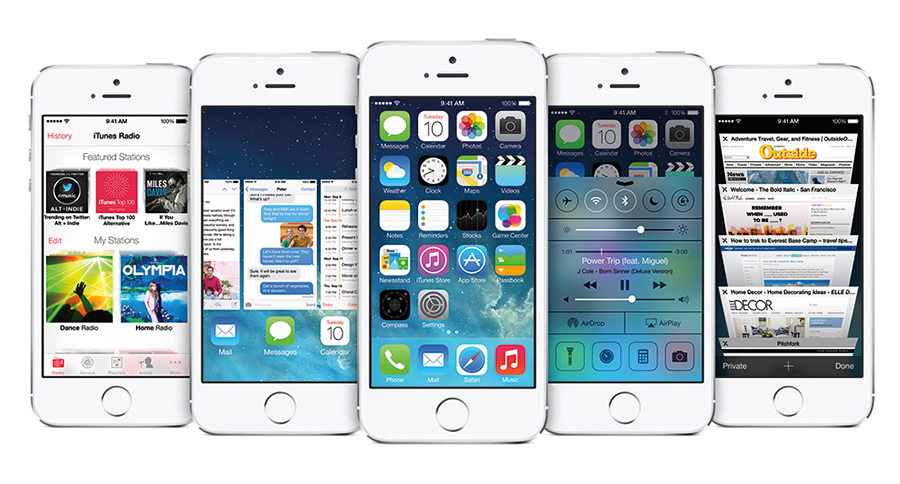
\includegraphics[scale=1.3]{img/ios-7.jpg}
	\end{figure}
\end{frame}
%--------------------------------------------------------------------------------%


%--% Arquitectura %--------------------------------------------------------------%
\begin{frame}
\frametitle{\ioslogo}
\framesubtitle{Arquitectura}
	
	iOS usa una arquitectura por capas, cada capa usa un interfaz provista por la capa anterior a ella. Las capaz mas bajas contienen servicios y tecnologías fundamentales. Las capas mas altas usan las abstracciones e interfaces provistas por las capas mas bajas y proveen servicios mas sofisticados. Cada capa contiene un conjunto de frameworks que son usados por la capa superior.
\end{frame}

\begin{frame}
	\frametitle{\ioslogo}
	\framesubtitle{Arquitectura}
	
	\begin{figure}[h]
		\centering
		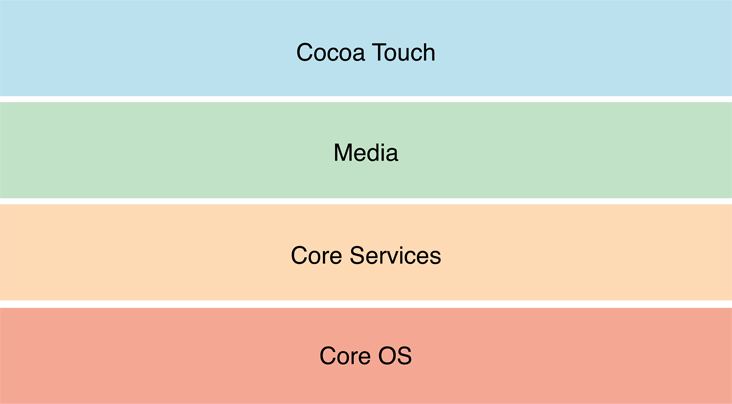
\includegraphics[scale=0.4]{img/layers.png}
	\end{figure}
\end{frame}

\begin{frame}
	\frametitle{\ioslogo}
	\framesubtitle{Arquitectura}
	
	\begin{itemize}
		\item{
			\textbf{Cocoa Touch}: Contiene frameworks para construir aplicaciones para iOS. Incluye soporte para el multitarea, entrada touch, notificaciones y otros servicios de alto nivel.
		}
		\vspace{1cm}
		\item{
			\textbf{Media}: Contiene los servicios e interfaces necesarias para video, graficos, y audio. Presenta varias clases por las cual facilita el mostrar o generar contenido multimedia.
		}
	\end{itemize}
\end{frame}

\begin{frame}
	\frametitle{\ioslogo}
	\framesubtitle{Arquitectura}
	
	\begin{itemize}
		\item{
			\textbf{Core Services}: Contiene servicios fundamentales para las aplicaciones, como los servicios de localización, iCloud, entre otros.
		}
		\vspace{1cm}
		\item{
			\textbf{Core OS}: Contiene todas las características de bajo nivel usadas por las demas capas. Maneja servicios fundamentales del sistema operativo como los hilos, administración de memoria, manejo del sistema de archivos.
		}
	\end{itemize}
\end{frame}
%--------------------------------------------------------------------------------%



%--% Planificacion %-----------------------------------------------%
\begin{frame}
\frametitle{\ioslogo}
\framesubtitle{Planificacion}
	El algoritmo de planificacion, es uno basado en colas multinivel con prioridades, cuyas prioridades estan divididas en 4 clases:
	
	\vspace{1cm}
	\centering
	\begin{tabular}{|c|c|} \hline
		Prioridad & Características \\ \hline\hline
		Normal & Hilos con prioridad no importante \\ \hline
		Alta & Prioridad mayor a la normal \\ \hline
		Modo Kernel & Hilos que fueron creados dentro del kernel \\ \hline
		Tiempo Real & Deben ser completados en un tiempo.\\ \hline
	\end{tabular}
\end{frame}
%--------------------------------------------------------------------------------%



%--% Sincronizacion %--------------------------------------------------------------%
\begin{frame}
	\frametitle{\ioslogo}
	\framesubtitle{Sincronizacion}
	
		iOS nos brinda y utiliza varios mecanismos de sincronización, entre algunos tenemos:
	\begin{itemize}
		\item \textbf{Atomic Operations}
		\item \textbf{Locks}
		\item \textbf{Condition Variables}
	\end{itemize}
\end{frame}

\begin{frame}
	\frametitle{\ioslogo}
	\framesubtitle{Sincronizacion}
	
	\textbf{Atomic Operations}: Contiene servicios fundamentales para las aplicaciones, como los servicios de localización, iCloud, entre otros. Normalmente se usan para operaciones simples o cortas.
	
	\begin{figure}[h]
		\centering
		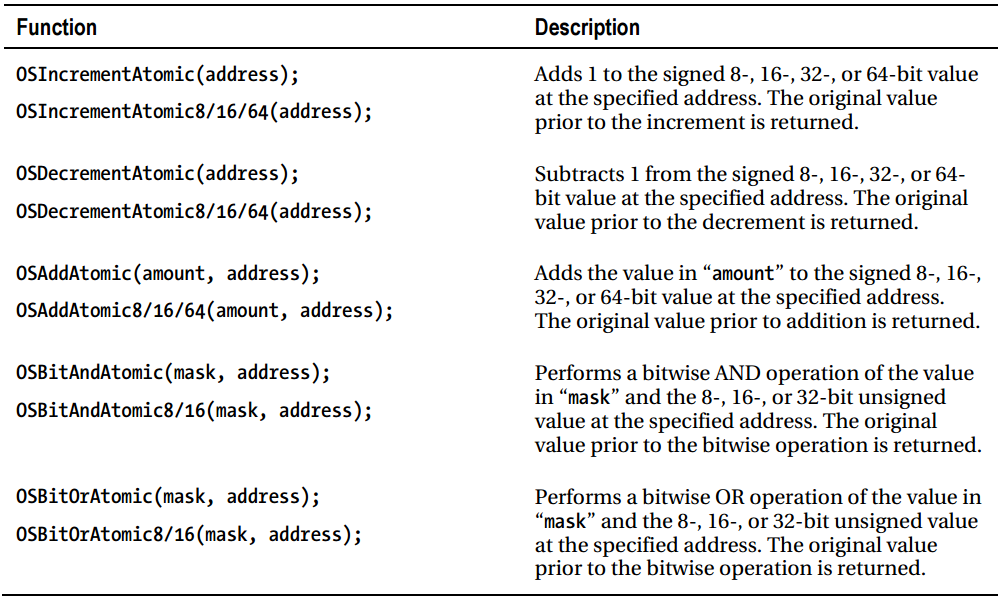
\includegraphics[scale=0.35]{img/operaciones_atomicas.png}
	\end{figure}
\end{frame}

\begin{frame}
	\frametitle{\ioslogo}
	\framesubtitle{Sincronizacion}
	
	\textbf{Locks}: Usados cuando se necesita sincronizar instrucciones o operaciones mas complejas y grandes. Cuando se pone un Lock alrededor de una sección del código, solo un hilo a la vez tendrá acceso a esta sección. Entre los tipos de locks que provee, tenemos Mutex, Recursive Lock, Read-Write Lock, Spin Lock, entre otros.
\end{frame}

\begin{frame}
\frametitle{\ioslogo}
\framesubtitle{Sincronizacion}
	
	\textbf{Condition Variables}: Permite la sincronización entre múltiples hilos proveyendo un mecanismo por el cual un hilo puede suspender sus ejecución hasta que una condición en particular (o evento) se cumpla, cuando esto ocurre se manda una señal o mensaje a los hilos que esperan por esto.
\end{frame}
%--------------------------------------------------------------------------------%



%--% Comunicacion %-----------------------------------------------%
\begin{frame}
\frametitle{\ioslogo}
\framesubtitle{Comunicación}
	El SDK de iOS y los frameworks que nos brindan las capas del sistema operativo, nos permiten realizar comunicación entre distintas aplicaciones de distintas formas, una es a traves de Airdrop, o definir esquemas de URL personalizados para enviar información.
\end{frame}
%--------------------------------------------------------------------------------%



%--% Administracion de la Memoria %-----------------------------------------------%
\begin{frame}
\frametitle{\ioslogo}
\framesubtitle{Administracion de la Memoria}
	
	El kernel XNU sigue el estado de la memoria física usando una estructura \texttt{vm\_page}. Existe una \texttt{vm\_page} por cada pagina física en memoria. Las paginas disponibles forman parte de una de las siguientes listas:
	
	\begin{itemize}
		\item \textbf{Active List}: Contiene las paginas físicas que están asignadas aunque sea a un espacio de direcciones virtuales y han sido usadas recientemente.
		
		\item \textbf{Inactive List}: Contiene las paginas que están asignadas pero no han sido usadas recientemente.
		
		\item \textbf{Free List}: Contiene las paginas no asignadas.
	\end{itemize}
\end{frame}

\begin{frame}
\frametitle{\ioslogo}
\framesubtitle{Administracion de la Memoria}

	El kernel enviara una señal al demonio pageout si detecta que el numero de paginas disponibles esta por debajo de un limite. En este caso se sacaran paginas de la lista de paginas no activas (Inactive List) con un algoritmo basado en LRU.
\end{frame}

\begin{frame}
\frametitle{\ioslogo}
\framesubtitle{Administracion de la Memoria}
	
	Cuando hablamos del desarrollo de apps para iOS, nos proveen dos metodos para el manejo de memoria en la aplicación.
	
	\begin{figure}[h]
		\centering
		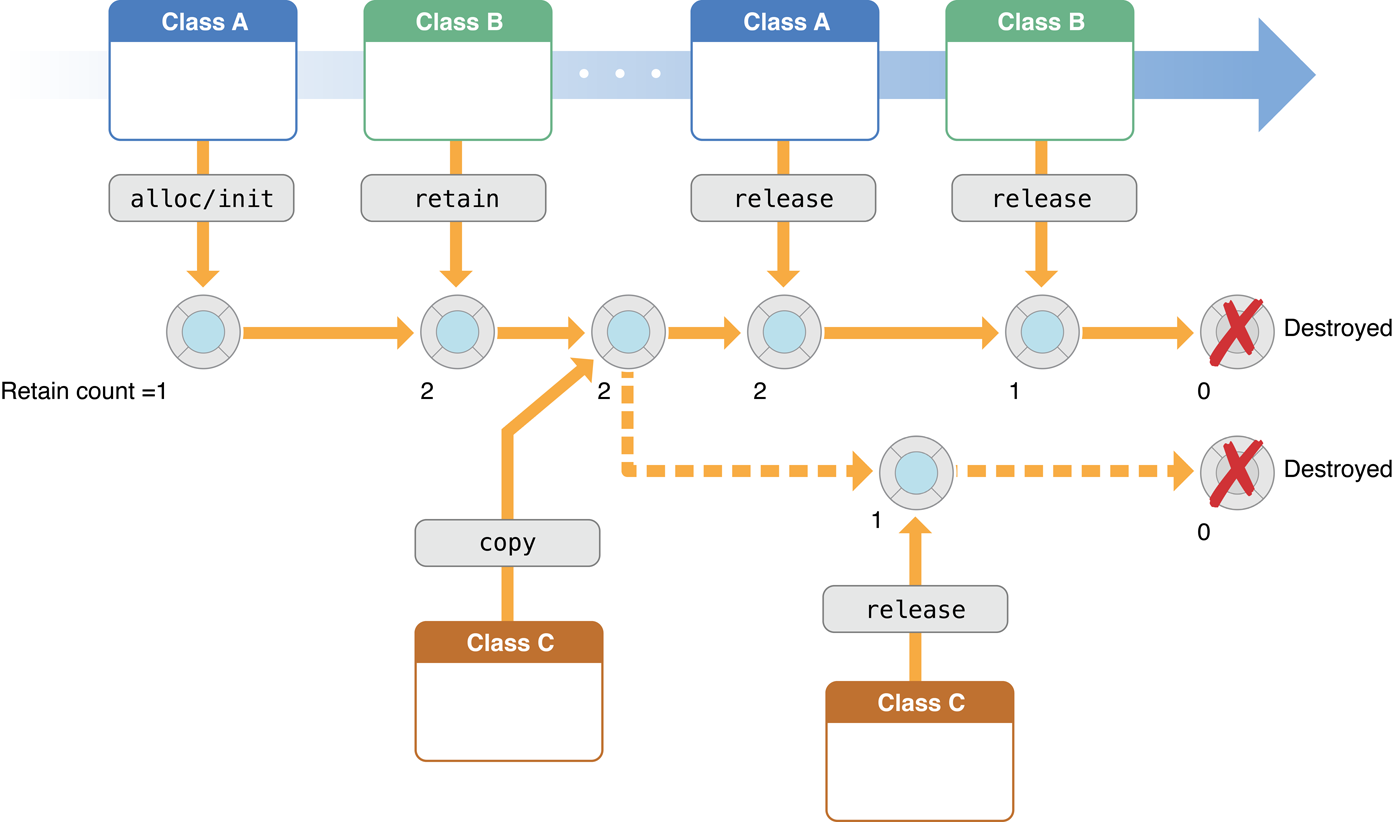
\includegraphics[scale=0.2]{img/memory_management.png}
	\end{figure}	
\end{frame}

\begin{frame}
\frametitle{\ioslogo}
\framesubtitle{Administracion de la Memoria}
	\begin{itemize}
		\item \textbf{MRR (Manuel retain-release)}: Explícitamente se maneja la memoria, llevando la cuenta de los objetos que se han creado.
		
		\item \textbf{ARC (Automatic Reference Counting)}: No hace falta llamar a las funciones de manejo de memoria explícitamente, al compilar el código automáticamente se insertan las llamadas a las funciones de manejo de memoria necesarias. Tiene los beneficios de la Recolección de Basura pero sin los costos de rendimiento de la misma.
	\end{itemize}
\end{frame}
%--------------------------------------------------------------------------------%


%--% Administracion de Dispositivos %-----------------------------------------------%
\begin{frame}
	\frametitle{\ioslogo}
	\framesubtitle{Administracion de los Dispositivos}
	
	Mientras que la capa mas alta de ese sistema operativo (Cocoa Touch) se encarga de manejar la entrada tactil, la capa de Media nos da acceso de alto nivel a la pantalla y el sonido, las capas mas bajas nos brindan una interfaz mas cercana al Hardware.
\end{frame}
%--------------------------------------------------------------------------------%


%--% Administracion de Archivos %-----------------------------------------------%
\begin{frame}
	\frametitle{\ioslogo}
	\framesubtitle{Administracion de los Archivos}

	El sistema de archivos del kernel XNU se basa en el diseño de VFS (Virtual File System), el cual se caracteriza porque nos permite añadir fácilmente nuevos sistemas de ficheros, así como añadir capas a un sistema de archivo existentes (compresión, encriptación). Los archivos y carpetas son representadas por una estructura \texttt{vnode}. Existe un \texttt{vnode} por cada archivo activo en el kernel.
\end{frame}

\begin{frame}
	\frametitle{\ioslogo}
	\framesubtitle{Administracion de los Archivos}
	
	Tenemos que iOS soporta distintos sistemas de archivos, HFS+, HFS, UFS, NFS, SMB, UDF y AFP. El sistema de archivos primario de iOS es HFS+. Este sistema de archivos es robusto contra eventos como fallas de poder o falles del kernel, la información puede ser traída al estado en donde se encontraba para tener al sistema de archivos en un estado consistente.
	
\end{frame}

\begin{frame}
\frametitle{\ioslogo}
\framesubtitle{Administracion de los Archivos}

	Y como el sistema de archivos de iOS esta basado en el de UNIX, cada objeto del sistema de archivos tiene un conjunto de permisologias de UNIX definidas por 3 atributos:
	\begin{itemize}
		\item \textbf{UID}: El id del usuario, el dueño del archivo.
		\item \textbf{GID}: El id del grupo.
		\item \textbf{UID}: Bits para indicar permisos y otros atributos.
	\end{itemize}
\end{frame}
%--------------------------------------------------------------------------------%


%--% Seguridad y Protección %-----------------------------------------------%
\begin{frame}
	\frametitle{\ioslogo}
	\framesubtitle{Seguridad y Protección}
	
	iOS brinda ciertas características interesantes cuando hablamos de protección, por ejemplo permiten que el usuario remotamente con su cuenta de iCloud pueda localizar su dispositivo, revisar alguna información en este, e incluso borrar toda la información en caso de robo.

	iOS encripta todos los archivos del sistema, para poder realizar un borrado rápido de toda la información en caso de que sea necesario.
\end{frame}
%--------------------------------------------------------------------------------%

\begin{frame}
\frametitle{\ioslogo}
\framesubtitle{Información Adicional}
	En el desarrollo de iOS, Apple siempre pone primero al usuario, y por lo tanto versión a versión ha mejorado su UX (User Experience) de gran manera. En este sistema operativo la facilidad de uso para el usuario y la fluidez a la hora de realizar cualquier tarea son detalles clave.
	
	Tambien, al Apple desarrollar este OS para un Hardware limitado, han podido optimizarlo en gran manera.
\end{frame}

%--% Bibliografia %--------------%
% \begin{frame}[t,allowframebreaks]
%	\frametitle{Referencias}
%	\nocite{memory}
%	\bibliographystyle{amsalpha}
%	\bibliography{bibliography.bib}
% \end{frame}


\end{document}
